\documentclass{article}
\usepackage[utf8]{inputenc}
\usepackage{graphicx}
\usepackage{titlepic}
\usepackage{hyperref}
\usepackage{xcolor}
\usepackage{amsmath}
\usepackage{textcomp}

\titlepic{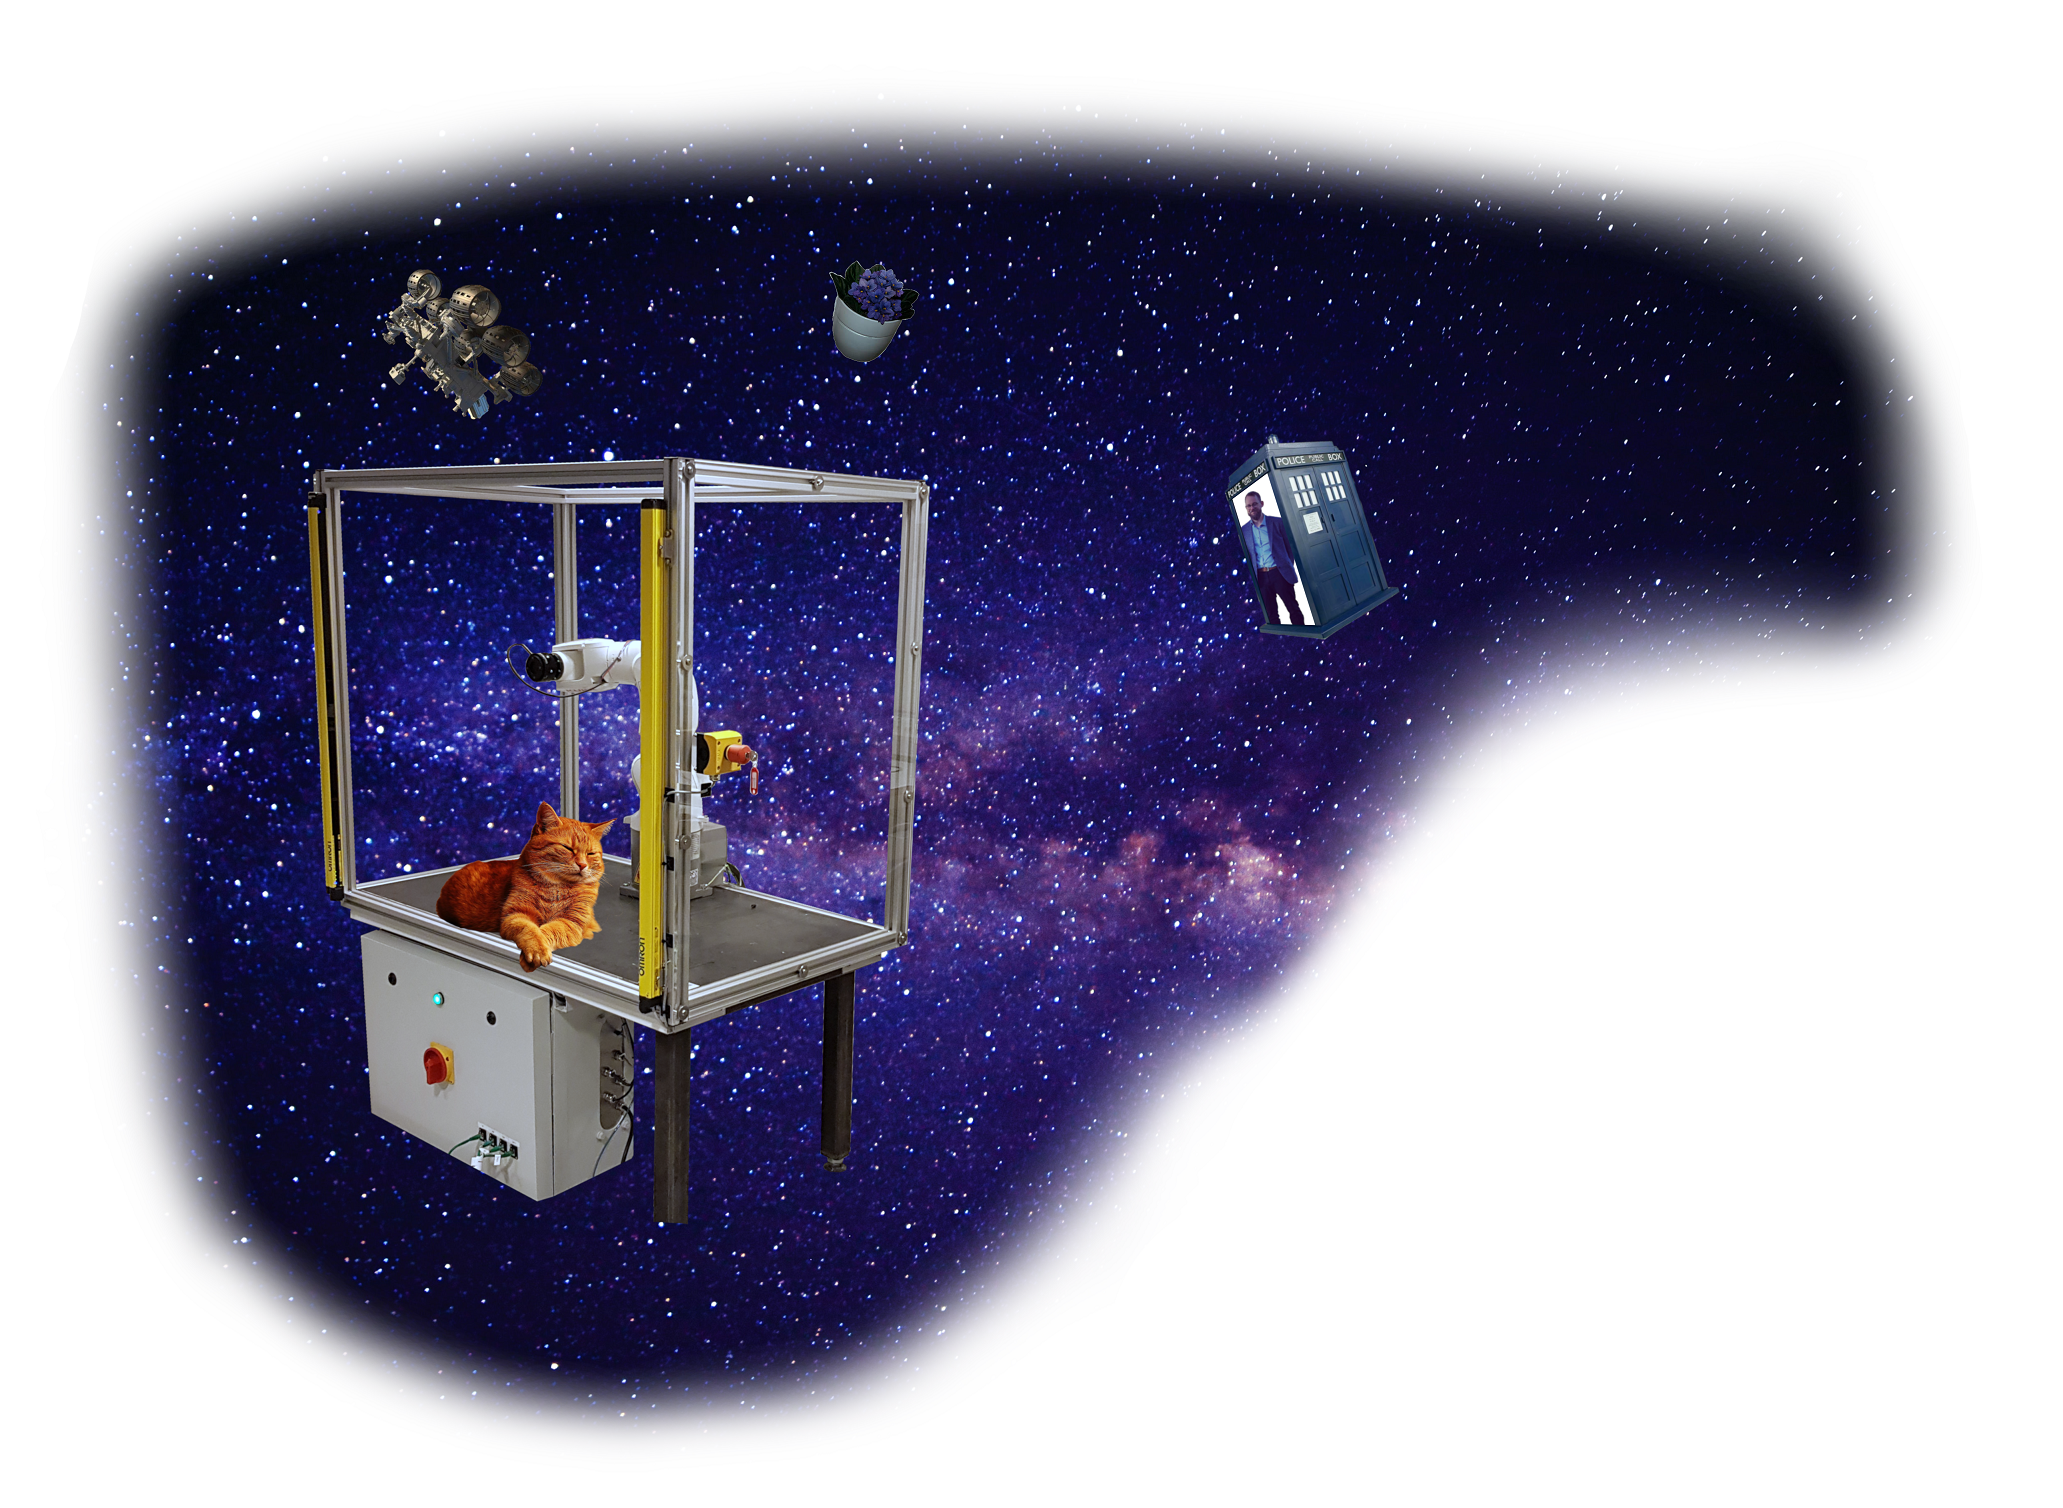
\includegraphics[width=\textwidth]{Pictures/robotlab1_croped.png}}
\title{Getting started with Kuka Robot Cell}
\author{Espen Teigen}
\date{March 2019}


\begin{document}

\maketitle

    Github: https://github.com/EspenTeigen/Kuka-KR-C4-commissioning

\newpage
\tableofcontents{}
\newpage


\section{Robot System Diagram}
    \begin{figure}[!h]
        \centering
        \includegraphics[scale=0.3]{"Pictures/Chart".png}
        \caption{System overview. It is not how everything is wired, but conceptual how it connects}
    \end{figure}

\newpage
\section{A brief overview of the Robot-cell and it's parts}
    \subsection{Manipulator}
    
     \begin{figure}[!h]
        \centering
        \includegraphics[scale=0.09]{"Pictures/KR_3_AGILUS".jpg}
        \caption{Kuka KR 3 R540 Agilus}
    \end{figure}
    
    
    Ahh... The manipulator, the part that everyone thinks is the robot, but, no. A robot consists of a controller, end-effector and a manipulator, but I am getting ahead of myself.
    \\\\
    The manipulator is the part that delivers the movement of the tool. In it self, it is just a collection of motors and joints, or as the robotics companies like to say "jointed-arm kinematic system". 
    \\\\
    The manipulator has four pneumatic(input/outputs) near the end-effector. It has an eight-pin M12 contact on the head, where I have used four of the pins on a force torque sensor.  
    
   
    \newpage
    \textcolor{blue}{\textbf{This manipulator is:}
    \begin{itemize}
        \item 6-axis
        \item Capable of moving 3kg of mass(included tool)
        \item Giving a $\pm 0.02mm$ pose repeatabillity
        \item Weighing 26.5kg without a tool
        \item Not very big. It has a maximum reach of 541mm(without tool)
        \item Silent, less then 68dB
        \item Made for pairing with the KR C4 compact controller
        \item What we would call an assembly robot
        \item Really, really fast(See KR 3 R540 Operating Instructions page 12)
        \item In my opinion, really good looking
    \end{itemize}}

    \textcolor{red}{\textbf{It is not:}
    \begin{itemize}
        \item A pot of petunias falling to the ground
        \item \textbf{A toy. When the manipulator is moving at full speed, it has the power to do some major damage to both humans and equipment. Never try to override the safety system, and keep body parts away from the robot cell. Try to avoid standing in front of the robot cell when the robot system are in operation, if you are not sure about how the robot is moving}
         \item A TARDIS\textsuperscript{TM} traveling in wibbly wobbly timey wimey space. 
    \end{itemize}}

     \textbf{In the back of the manipulator you will find:}
    \begin{itemize}
        \item Air 1-4
        \item X32, this connector is used for mastering(calibrating) the robot
        \item X76, this connector is used for transferring power and data to the connector on the head of the manipulator
        \item One thick cable(X20), used for transferring power to the motors
        \item One thin cable(X21) used for data communication from the controller to the robot. 
        \item One ground wire, used for equipotential bonding with the controller. 
    \end{itemize}
    
  \newpage
  
        \subsubsection{Force-torque sensor}
        \begin{figure}[!h]
            \centering
            \includegraphics[scale=0.2]{"Pictures/FT300".png}
            \caption{Robotiq FT-300}
        \end{figure}
        
        As the section name implies, this is a force-torque sensor. It gives us 3-axis of force, and 3-axis of torque. 
        
          \begin{figure}[!h]
            \centering
            \includegraphics[scale=0.5]{"Pictures/FT300-diagram".png}
            \caption{Axis of sensitivity}
        \end{figure}
        This gives us the possibility to give the robot a feeling of touch. The FT-300 is placed between the manipulator and end-effector.
        \\\\
        This sensor is sending it's data via modbus to a PLC, that transfers the data to the robot system.
       
\newpage
        
        \subsubsection{Pneumatic's}
        The pneumatics on the robot is made of three part. 
        \begin{figure}[!h]
            \centering
            \includegraphics[scale=0.5]{"Pictures/stanley fatmax OL244".jpg}
            \caption{An Stanley Fatmax OL244 air compressor with pressure regulator}
        \end{figure}
        
        \begin{figure}[!h]
            \centering
            \includegraphics[scale=0.3]{"Pictures/festo".jpg}
            \caption{A 5/2 mono-stable solenoid valve}
        \end{figure}
        
        \begin{figure}[!h]
            \centering
            \includegraphics[scale=0.5]{"Pictures/cylinder".jpg}
            \caption{A SMC CD55N12 pneumatic cylinder}
        \end{figure}
        
        \begin{figure}[!h]
            \centering
            \includegraphics[scale=0.5]{"Pictures/air-flow valve".jpg}
            \caption{And two SMC air-flow valves(not to scale, its really small)}
        \end{figure}
        
\newpage

        This setup makes it possible to control the pneumatic valve with digital output 0 from the robot controller. Boolean TRUE extends the cylinder, and boolean FALSE retracts the cylinder. 
        \\\\
        The force of the cylinder is controlled with the pressure regulator on the air compressor. 
        \\\\
        The speed of the cylinder is controlled with the air-flow valves on the back of the manipulator. The one marked +, controls the retraction speed, and the other one controls the extension speed.
        \\\\
          Notice that the air-flow regulators has a check valve that lets air inn to the cylinder. This is because we want to restrict the air-flow out from the cylinder, and not in to it. If you restrict the airflow in, the cylinder will move like you are playing counter strike on a machine with 56k mode, it will lag. 
        
        \begin{figure}
            \centering
            \includegraphics[scale=1]{"Pictures/pneumatic schematic".png}
            \caption{Pneumatic schematic for control of pneumatic cylinder}
        \end{figure}
    
\newpage

        \subsection{Robot Controller}
        
        \begin{figure}[!h]
            \centering
            \includegraphics[scale=0.4]{"Pictures/kr c4 compact".jpg}
            \caption{KR C4 compact}
        \end{figure}
        
        The heart and nerve of the robot system. It is on this one you write you're program, do all the configurations and so on. It reads the rotary encoders on the manipulator, and send control-signals to it. It also handles communication with other robot-controllers, PLC's and computers. It can control servo drives, so on and so forth. If you want to find out more of what it can do, i suggest that you have a look in the documentation; KR C4 compact, Operating Instructions(You can find this on the KRC4 docs standard disk, or on kuka's download center.
        \\\\
        This specific controller has some options that are important to mention. We have the KRC4 compact DC4 FSoE ECAT M/M X55 EN. That mean that this controller is equipped for use with EtherCAT-bus, and supports FSoE(Fail Safe over Ethernet)(made possible with Beckhoff EL6695-1001 Master/master EtherCAT-bridge).  X55 is the power connector to the EtherCAT-bridge inside the controller. I'll describe this under the sub-section EtherCAT further down in the document.
        
\newpage

        \subsubsection{Smart Pad}
        
        \begin{figure}[!h]
            \centering
            \includegraphics[scale=0.5]{"Pictures/smartpad".jpg}
            \caption{Kuka Smart Pad}
        \end{figure}
        
        The first line of interaction with the Kuka robot system. This is a touch pad with OK resolution and horrible touch interface(I suggest you use a Bluetooth keyboard and mouse if you are going to do a lot of work on it).
        \\\\
        But it shines when it comes to moving the robot manipulator. The 6-D mouse on the right side is actually nice to use when you get used to it. The interface is also quit intuitive(in certain areas). I will give a better description how to use it when i start rambling about starting the robot and programming.
        
        \newpage
        
        \subsubsection{PC-interface}
       To connect a PC to the controller, connect to the PC port on the control cabinet below the manipulator using a ethernet cable. 
        \\\\
        USefull information about PC interface:
        \begin{itemize}
            \item Connect you're PC to the PC port on the cabinet
            \item IP adresse of the controller: 172.31.1.147
            \item Subnet mask:                  255.255.0.0
            \item Default gateway:              0.0.0.0
            \item IP adresse of the PLC: 172.31.1.11 
        \end{itemize}
        The PLC is another part of the system i will explain more about it later. 
        \paragraph{Software}
         To do commissioning on the robot(add IO, modules etc.) and some programming of the robot, we use WorkVisual. It is a software made by Kuka, and are used for configuring robot cells. Usually, there is no need to use this software.
         
        \subsubsection{EtherCAT}
        Our controller is configured with the etherCAT and Fail Safe over EtherCAT(FSoE) option. EtherCAT is a real-time ethernet based industrial communication protocol, and is standardized in IEC 61158. It uses standard IEEE 802.3 ethernet as the physical layer without modification. 
        \\\\
        FSoE is a communication protocol that gives a SIL 3 safety system. This simplifies our connections, since we only need an ethernet-cable to enable all our safety related stuff like; light grid and emergency stop. 
        \\\\
        On the controller, you will find a plug without a cable that is plugged in to the X55-port. This is not a dummy plug, it is crucial. Inside the plug, there are some jumper-wires. They are put there to power the EtherCAT-bridge from an internal 24V supply. If this plug is removed, the safety communication will fail, and the robot won't move. There is a picture of how it is wired in the system design picture you can find on my Github under Kuka-KR-C4-commissioning.
        
        
\newpage

    \subsection{Control cabinet}
    The control cabinet is the storage for all the electronics, and a pneumatic valve. Inside there is a PLC, the robot controllers IO, power supply, fuses, relays and an ethernet switch.
        \subsubsection{Front panel}
        \begin{figure}[!h]
            \centering
            \includegraphics[scale=0.3]{"Pictures/cabinet_front".png}
            \caption{Front panel of control cabinet}
        \end{figure}
        
        \paragraph{Reset button}
        The reset button is used to acknowledge External Emergency Stop warnings after the light grid or the emergency stop button on the side of the robot cell has bin triggered. It is also used to remove communication error when after the system has been turned of. 
        
        \paragraph{Main Power Switch}
        This is used to turn of the power to the power supply, resulting in that everything is turned of. The only place with voltage in the system is on the input to the power switch.
        
        \paragraph{Communication interface}
        \textbf{PC}: This is where you will connect you're PC. In the cabinet, the PC port is connected to a Phoenix firewall, that is used as a switch at the moment. This switch is connected to the robot controller via X66 and to the programming interface on the PLC.
        \\\\
        \textbf{X65}: Is connected to X65 on the controller. This is is the IO's that the robot controller can control directly without the PLC.
        \\\\
        \textbf{X66}: Is the PC interface to the controller.
        \\\\
        \textbf{X67.1} Is the communication port from the PLC to the robot controller. We have a Beckhoff CX9020 embedded PC with a soft PLC on it, that communicates with a EL6695-1001 etherCAT Master/Master-bridge inside the robot controller. All safety communication and regular communication goes through this ethernet cable.  
        
        \newpage
        
        \subsection{Inside the control cabinet }
        \begin{figure}[!h]
            \centering
            \includegraphics[scale=0.2]{"Pictures/cabinet_inside".jpg}
            \caption{Inside the control cabinet}
        \end{figure}
        
        \begin{enumerate}
        
            \item The PLC, it handles all the safety, communication with robot controller and communication with the FT-300 sensor. 
            \item The robots IO, these are directly controlled from the robot controller, and can be interfaced in a robto program. Output 0 is used for controlling pneumatic valve.
            \item Ethernet firewall/switch that also is enabled for communication over mobile network.
            \item 5/2 pneumatic valve.
            \item 24V-DC, 10A power supply.
            \item Fuses; from left to right: PLC, Robot controller IO, Ethernet switch, light grid, 230V mains, FT-300. 
            \item Relays, the leftmost is used for the 5/2 valve, the second one is not used.
        \end{enumerate}
        
        \newpage
        
        \subsubsection{Embedded PC, PLC, Safety, IO}
        
        \begin{figure}[!h]
            \centering
            \includegraphics[scale = 0.3]{"Pictures/PLC".png}
            \caption{Embedded PC with IO's}
        \end{figure}
        
        The embedded PC handles PLC, safety and IO connections. It sends FSoE parameters to the robot controller, and also values from the force torque sensor.  
    
        \begin{itemize}
            \item The ethernet-plug on the left in the picture is the programming interface of the embedded PC
            \item The first yellow block, is safety-inputs(EL1904). On the top emergency stop and reset is connected, and in the bottom the light grid is connected with OSSD( Output Signal Switching Device, google it). 
            \item The second and third yellow block, is actually one block, and is safety outputs(EL2904). It is not in use at the moment, but is put there for further development. 
            \item The fourth block is the safety PLC, and it handles all the safety logic. There are no connections to ut, because everything is handled by the internal bus.
            \item The fifth bloc(The one with two RS485-plugs) is used to interface the FT-300 sensor.
            \item And the last one(EK1110) is an etherCAT-coupler, and is connected to the X67.1 port on the robot controller. 
        \end{itemize}
        
        \newpage
        
        \paragraph{Software}
        The software used for programming of the embedded PC is TwinCAT 3 XAE. It is a visual studio ad-on, and should be fairly intuitive to use for people with knowledge of the software. Of course, this does not mean that the ad-on is easy to use. I'll go further into the use of the software later. 
        
        \subsubsection{Robot IO}
        \begin{figure}[!h]
            \centering
            \includegraphics[scale=0.4]{"Pictures/IO".png}
            \caption{The robot's IO}
        \end{figure}
        
        The ethernet-cable on the left is connected to X67.1 and is on the robot controller's internal etherCAT bus. This means, that if more IO or other modules that the robot is to be needed, they can be added on to this one, and only need to be configured in Work Visual if Kuka has a DTM-file(device description file) for the module(otherwise you have to add the module on to the embedded PC and configure the communication, see my document \textbf{Sending-data-between-Beckhoff-PLC-and-Kuka-Robot-Controller-KRC4-} on my github page)..
        
        \newpage
        
        \paragraph{Robotiq Force-torque sensor}
        You can read about how the seonor works her:\\\\ https://robotiq.com/products/ft-300-force-torque-sensor?ref=nav\_product\_new\_button
        \\\\
        The sensor is connected to the EL6022 on the embedded PC, and uses ModBUS RTU as communication-protocoll. The embedded PC reads the 6 values and transfers it to the robot controller. On the controller you can find these values with the global names:
        \begin{itemize}
            \item ForceX
            \item ForceY
            \item ForceZ
            \item MomentX
            \item MomentY
            \item MomentZ
        \end{itemize}
        
        On the PLC inside the embedded PC(you can find it in TwinCAT3), there is a program called MAIN that handles the reading and sending of values to the controller. 
        
        \paragraph{Data transmission to and from controller}
        Se document \textbf{Sending-data-between-Beckhoff-PLC-and-Kuka-Robot-Controller-KRC4} on my github page. 

\newpage

    \subsection{Calibration of robot}
        To give the highest position repeatably, you have to do something Kuka calls "mastering". Mastering is done with the aid of a Micro electronic mastering device(MEMD). It should always be located in the cabinet on the robot lab(it is quite expensive, so be careful with it). 
        
        
        \begin{figure}[!h]
            \centering
            \includegraphics[scale=0.3]{"Pictures/memd_suitcase".jpg}
            \caption{The MEMD suitcase}
        \end{figure}
        
        \begin{figure}[!h]
            \centering
            \includegraphics[scale=0.5]{"Pictures/memd".jpg}
            \caption{The MEMD}
        \end{figure}
        
        There is no need to do mastering often, 1-2 times a year should suffice, exceptions are if the manipulator has crashes or if the robot cell has been moved, and you need the high precision. Also, if you are working with high loads(1-2)Kg, mastering has to be done. You have something called EMD mastering with load correction. 
        \\\\
        Important: If mastering should be done, previous mastering has to be deleted first. 
        \\\\
        You can find videos about mastering on YouTube, so i will not use to much time on it. It is easy to do. 
        
        \newpage

    \subsection{Safety and maintenance}
        \subsubsection{Do's }
        \textbf{Every time the robot is used}
        \begin{itemize}
            \item That there are no loose parts that can fall off during operation.
            \item Listen for sounds that should not be there.
            \item Make sure the people using the robot is properly trained.
            \item That there is no cat's inside the control cabinet(those pesky critters can get in anywhere. Reference "On the rheology of cats. M.A. Fardin, Rheology Bulletin, 83(2) July 2014")
            \item When finished, turn off robot controller from the teach pendant, and not the power button.
        \end{itemize}
        
        \textbf{Once a month}
        \begin{itemize}
            \item Check that there is no damage to the wires and hoses.
            \item Check that the bolts on the base of the manipulator is tight. 
            \item Check that the bolts on the light grid is tight.
            \item Check that the bolts on the plexi-glass is tight.
            \item Look at my masterpiece in awe.
        \end{itemize}
        
        \textbf{Every sixth month}
        \begin{itemize}
            \item Master the robot.
            \item Remove covers on manipulator and check that the belts are intact and tight, remove dust.
            \item Open controller and remove dust. 
            \item Check oil level in compressor.
            \item Test that the safety equipment work properly.
        \end{itemize}
        
        \subsubsection{Emergency stop's}
        There is two emergency stops on the robot. One on the teach pendant. The warning from this one can be cleared from the teach pendant. The other one is on the right side og the robot cell, and the warning can only be cleared from the reset button on the cabinet.
        
        \newpage
        
        \subsubsection{Light grid}
        The light grid, is the yellow bars on each side of th robot cell. They are rated SIL 3, and are approved for safety use. 
        
        \paragraph{Bluetooth}
        The light grid is equipped with Bluetooth monitoring and configuration, and the software to be used are SD manager 2 from Omron.
        
        \paragraph{Muting}
        The light grid is equipped with muting, this makes it possible to turn off the light grid with other equipent. This option is not configured at the moment, but it is accessable. Have a look in the Omron F3SG-RA user manual. 
        \\\\
        \textbf{\textcolor{red}{Important:}} To maintain the safety of the system, proper care has to be taken. 
        \begin{itemize}
            \item  Do never use non-safety equipment to control the muting.
            \item Never give humans a physical way to mute the light grid(like a button).
            \item Do a risk-assessment before muting is an option, always. 
            \item Consider other options before muting is chosen.
            \item Consider using extra safety equipment to maintain a high level of safety.
            \item The Kuka manipulator should never be in motion when light grid is muted.
            \item You can use the available safety outputs to mute the light grid.
        \end{itemize}

        My recommendation is that you program the Safety PLC in TwinCAT3 to send a \textbf{Safe Operational stop signal} to the controller
        \\
        (Refer to KR\_C4\_EtherCAT\_Bridge\_FSoE\_Master\_master\_en.pdf document; page 19), before the light grid is muted, and release the Safe Operational stop signal after the muting is turned off. In this way, the manipulator can not move while the muting is enabled. 
        \\\\
        \textbf{\textcolor{red}{In a chain of safety-equipment, there should never be non-safety equipment, that includes relays, IO's and switches}}
        
        \newpage 
        
\section{Getting started}
    \subsection{Get everything connected}
    \begin{itemize}
        \item Air from compressor(If pneumatic cylinder is used).
        \item Power to cabinet.
        \item Power to robot controller.
        \item power and data cable from controller to manipulator.
        \item Data cables: PC, X65, X66 and X67.1 is connected to appropriate places, PC can be excluded if no computer is being used.
        \item smartPad is connected to controller
        \item If computer is being used: IP-address and subnet mask is in correct range.
    \end{itemize}
    
    \subsection{Powering up the system}
    \begin{enumerate}
        \item Turn power on cabinet on robot cell first. Wait 15-30 seconds so the PLC can boot up.
        \item Turn power on robot controller.
        \item Get coffee while controller is booting.
        \item Push reset button.
        \item Push and release emergency stop button on robot cell.
        \item Push reset button again.
        \item If communication error KRC4 primary error sustains, jump to(not literary) \textbf{Problems resetting communication error warning on SmartPad} 
    \end{enumerate}
    \subsubsection{Problems resetting communication error warning on SmartPad}
    At the time of writing this, we do not have a license for some of the library's used on the TwinCat 3 system. But Beckhoff has a one week free license-trial, and that is what I've been using. To renew the license's, open the TwinCAT project kuka\_robot\_project\_twinsafe\_modbus.sln(you can find this on my github page). If changes has been done on the project after my departure, use that project instead. 
    \\\\\
    \begin{figure}[!h]
        \centering
        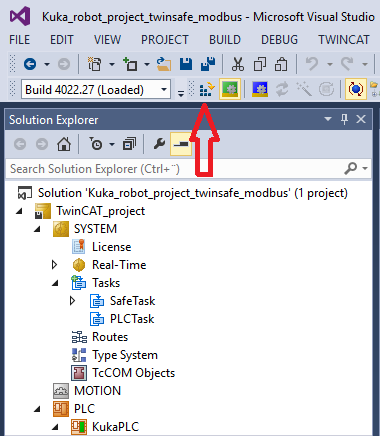
\includegraphics[width=\textwidth]{Pictures/twincat_upload_installation.png}
        \caption{Push the upload button, pretty please}
        \end{figure}
    By pushing the button, you will download the project to the embedded PC, if you're licenses is old and musky, TwinCAT will ask if you want to renew the license, follow the instructions. 
    \\\\
    After the download is done, push the reset-button on the cabinet. It should hopefully remove the error, and all you have to do is acknowledge that the error has been there.  

\newpage

\section{\textbf{\textcolor{red}{IMPORTANT, READ THIS!}}}
On the SmartPad, you have a menu under $$Start-up->Network Configuration->Internal subnets$$. 
\textbf{\textcolor{red}{Never change anything here. This are the buses used between components in the controller. Changes here will brick the controller, and you need to order a recovery stick from Kuka to re-install everything. I repeat, NEVER DO CHANGES HERE}}. 
\\\\
For some reason, this menu is easy accessible for everyone logged in as expert or higher.

\newpage 

\section{Wiring diagrams}

    \subsection{Power distributions}
    
    \begin{figure}[!h]
        \centering
        \includegraphics[width=\textwidth]{"Pictures/power-supply diagram".png}
        \caption{The fuses are rated for power consumption at current moment. If fuses should start breaking for no apparent reason after adding more IO's and modules, it is possible they should be bigger}
    \end{figure}
    
    \newpage
    
     \subsection{Robotiq FT-300}
    
    \begin{figure}[!h]
        \centering
        \includegraphics[width=\textwidth]{"Pictures/FT-300-Wiring".png}
        \caption{Figure is a modified version of schematic from Kuka KR AGILUS sixx KR 3 R540 operating instructions, version BA KR AGILUS sixx MSR V1 page 48}
        \label{fig:my_label}
    \end{figure}
    
    \newpage
    
    \subsection{Beckhoff CX9020}
    \subsubsection{EL1904}
    
    \begin{figure}[!h]
        \centering
        \includegraphics[width=\textwidth]{"Pictures/CX9020-EL1904".png}
        \caption{Wiring of El1904-module}
    \end{figure}
    
    \newpage
    
    \subsection{Beckhoff EK1100}
    \subsubsection{EL2809}
    
    \begin{figure}[!h]
        \centering
        \includegraphics[width=\textwidth]{"Pictures/EL2809".png}
        \caption{K1 is used for pneumatic valve, K2 is available for further use}
    \end{figure}
    
    \newpage
    
    \subsection{Omron F3SG-RA}
    
    \begin{figure}[!h]
        \centering
        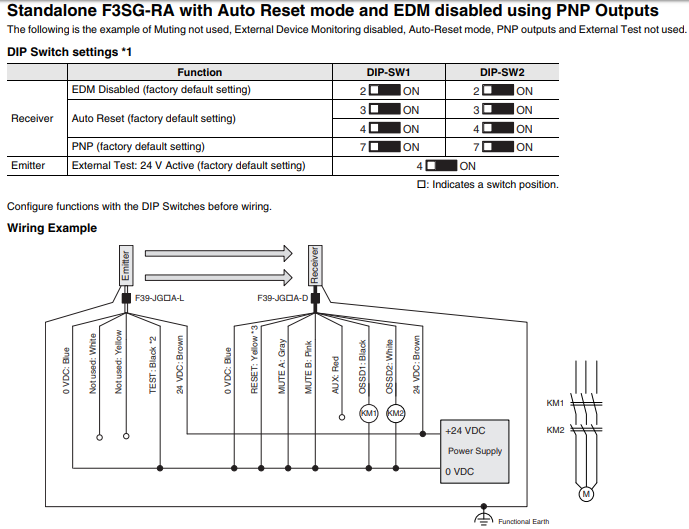
\includegraphics[width=\textwidth]{Pictures/F3SG-RA.png}
        \caption{Diagram is borrowed from Omron F3SG-RA Series Family Datasheet}
        \label{fig:my_label}
    \end{figure}
    
 
    
    
        
\end{document}